\chapter{Methodology}\label{ch:method}

	\section{PDR Implementation} \label{sec:method_PDR}
    
    	As defined in Section \ref{ch:intro}, the design of the indoor positioning system is constrained to the android smart-phone environment. As identified in the literature review a PDR system consists of a simple cycle:
          \begin{enumerate}
            \item identify subsets of the data corresponding to individual step;
            \item estimate the length of the step; and
            \item estimate the step heading or change in heading.
          \end{enumerate}
          
         For the android environment, the PDR design is described in Figure \ref{fig:method_PDRflow}.
         \begin{figure}[t]
           \centering        
           \fbox{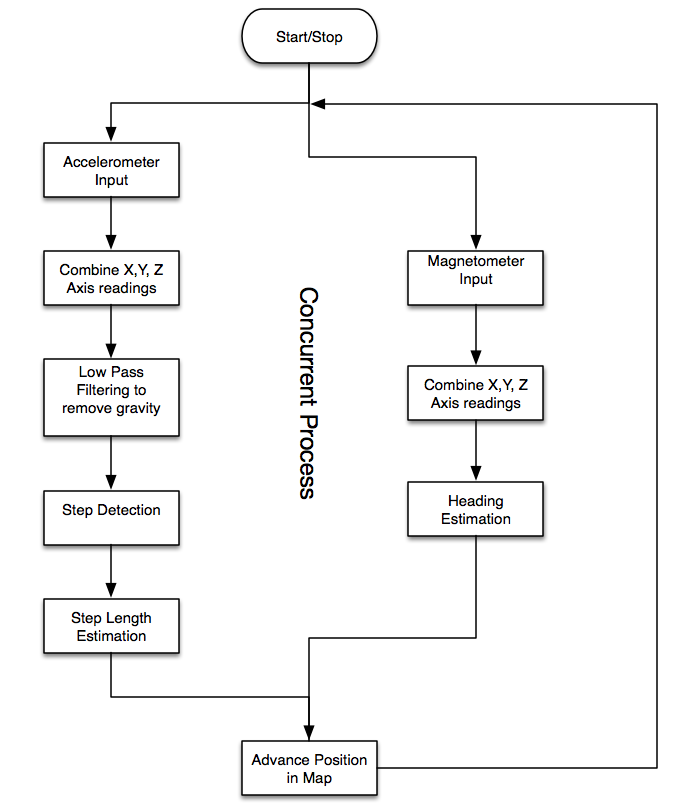
\includegraphics[scale=0.5]{PDRflow}}
           \caption{PDR Implementation}
           \label{fig:method_PDRflow}
         \end{figure}
    
    	%\subsection{Step Detection} 
        
       % \subsection{Step Length Calculation}
        
        %\subsection{Heading Estimation}
        
        % heading + step
        
    \section{Experimental Methods} \label{ssec:method_DR_experiment}
    
          Experiments conducted so far have revolved around identifying an accurate PDR system. Hence, the experiments described below verify the PDR cycle.
        
          \subsection{Step Detection Experiment}
          The step detection experiment will be conducted to verify that the algorithm implemented correctly detects a step. The user will walk a pre-defined number of steps with the smart-phone. The accelerometer data readings will be saved and the algorithm will be applied to the data. A correct system will be one that correctly identifies the number of steps taken. Appendix \ref{app:results} showcases preliminary results of the conducted experiment.

          \subsection{Step Length Experiment}
          
          The step length experiment will be conducted to verify the correct distance walked by the user. The user will walk in a straight line for a pre-defined distance in metres. The accelerometer data readings will be saved and the algorithm will be applied to the data. A correct system will be one that correctly calculates the distance walked.

          \subsection{Map Matching Experiment}
          To test the complete PDR cycle,i.e., step detection, step length, heading estimation and experiment will be conducted where the user walks in a pre-defined path in the environment. The PDR algorithms will then be applied to the saved sensor readings and a historical path will be formed. The accuracy of the PDR system can be quantified by comparing the PDR path to the correct path. Appendix \ref{app:results} showcases preliminary results of the conducted experiment.